\documentclass[]{article}

% Imported Packages
%------------------------------------------------------------------------------
\usepackage{amssymb}
\usepackage{amstext}
\usepackage{amsthm}
\usepackage{amsmath}
\usepackage{enumerate}
\usepackage{fancyhdr}
\usepackage[margin=1in]{geometry}
\usepackage{graphicx}
%\usepackage{extarrows}
%\usepackage{setspace}
%\usepackage{xcolor}
\usepackage{color}
\graphicspath{ {./images/} }
%------------------------------------------------------------------------------

% Header and Footer
%------------------------------------------------------------------------------
\pagestyle{plain}  
\renewcommand\headrulewidth{0.4pt}                                      
\renewcommand\footrulewidth{0.4pt}                                    
%------------------------------------------------------------------------------

% Title Details
%------------------------------------------------------------------------------
\title{Deliverable \#1 Template : Software Requirement Specification (SRS)}
\author{SE 3A04: Software Design II -- Large System Design}
\date{}
                            
%------------------------------------------------------------------------------

% Document
%------------------------------------------------------------------------------
\begin{document}

\maketitle
\noindent{\bf Tutorial Number:} T03\\
{\bf Group Number:} G06 \\
{\bf Group Members:}
\begin{itemize}
	\item Virochaan Ravichandran Gowri
	\item Alex Yoon
	\item Noah Goldschmied
	\item Krish Dogra
	\item Leo Vugert
\end{itemize}

\section*{IMPORTANT NOTES}
\begin{itemize}
	\item Be sure to include all sections of the template in your document regardless whether you have something to write for each or not
	      \begin{itemize}
		      \item If you do not have anything to write in a section, indicate this by the \emph{N/A}, \emph{void}, \emph{none}, etc.
	      \end{itemize}
	\item Uniquely number each of your requirements for easy identification and cross-referencing
	\item Highlight terms that are defined in Section~1.3 (\textbf{Definitions, Acronyms, and Abbreviations}) with \textbf{bold}, \emph{italic} or \underline{underline}
	\item For Deliverable 1, please highlight, in some fashion, all (you may have more than one) creative and innovative features. Your creative and innovative features will generally be described in Section~2.2 (\textbf{Product Functions}), but it will depend on the type of creative or innovative features you are including.
\end{itemize}

\newpage
\section{Introduction}
\label{sec:introduction}
% Begin Section

\subsection{Purpose}
\label{sub:purpose}
% Begin SubSection
This Software Requirement Specification has been created to specify the requirements needed to develop a secure communication app (VanklComm) for our organization. This SRS will ensure to cover functional requirements specifying how the app will perform the secure communication, including viewpoints from stakeholders and common business events and use cases and non-functional requirements outlining specifications of the system. Red text indicates a creative feature that goes beyond the project specifications.
% End SubSection

\subsection{Scope}
\label{sub:scope}
% Begin SubSection
\par The software product that will be produced is VanklComm, a secure chat application on Android. The product will allow for all employees of a company to communicate in a secure fashion, while also storing all texts in a database for security.
\\
\par \noindent Users will be required to create an account on VanklComm and be verified by their company in order to begin chatting. The main function of the product is the person-to-person chat, however there will also be \textcolor{red}{announcement boards} that managers can use to notify all of their employees.
\\
\par \noindent An objective of the software is to provide companies with secure chatting that prevents espionage from employees. Another objective of the software is that it must be easy to use, so that employees will have an easy transition over to the service. The last objective of the software is the encryption service. The software will provide end-to-end encryption on messages sent and received, which is what provides the secure chat.

% End SubSection

\subsection{Definitions, Acronyms, and Abbreviations}
\label{sub:definitions_acronyms_and_abbreviations}
% Begin SubSection
\begin{itemize}
	\item API – Application Programming Interface
	\item ASDK – Android Software Developer Kit
	\item KDC – Key Distribution Centre
	\item VanklComm – Viro-Alex-Noah-Krish-Leo communication

\end{itemize}
% End SubSection

\subsection{References}
\label{sub:references}
% Begin SubSection
\begin{itemize}
	\item[[1]] D. Nichols, “Coloring for Colorblindness,” Davidmathlogic.com, 2019.
	\\Available: https://davidmathlogic.com/colorblind/\#\%23D81B60-\%231E88E5-\%23FFC107-\%23004D40
	\item[[2]] FeDev, “Why is Dark Mode more than just a trend?,” Medium, Oct. 20, 2023.
	\\Available: https://bootcamp.uxdesign.cc/why-is-dark-mode-more-than-just-a-trend-224b8163acc6. Accessed: Feb. 14, 2024
	\item[[3]] Washington University in St.Louis, “Performance Analysis of Data Encryption Algorithms,” Wustl.edu, 2022.
	Available: https://www.cs.wustl.edu/\~jain/cse567-06/ftp/encryption\_perf
	\item[[4]] Oracle, “Response Time Analysis Made Easy in Oracle Database 10g,” Oracle.com, 2019.
	Available: https://www.oracle.com/technical-resources/articles/schumacher-analysis.html
	\item[[5]] GPS.gov, “GPS.gov: GPS Accuracy,” Gps.gov, 2019.
	\\Available: https://www.gps.gov/systems/gps/performance/accuracy
	\item[[6]] Federal Trade Commission, “Use Two-factor Authentication to Protect Your Accounts,” Consumer Advice, Sep. 12, 2022.
	Available: https://consumer.ftc.gov/articles/use-two-factor-authentication-protect-your-accounts\#:\~:text=Using\%20two\%2Dfactor\%20authentication\%20is
	\item[[7]] “99.999\% Uptime: Ensuring 5 Nines Uptime - Stratus Technologies,” Stratus | Zero-touch Edge Computing. Available: https://www.stratus.com/about/company-information/uptime-meter/
	\\\#:\~:text=Availability\%20is\%20normally\%20expressed\%20in
	\item[[8]] L. Shinder and M. Cross, “Understanding Cybercrime Prevention,” Scene of the Cybercrime, pp. 505–554, 2008, doi: 10.1016/B978-1-59749-276-8.00012-1.
	\item[[9]] “Google Play.” Accessed: Feb. 11, 2024. Online.
	Available: https://play.google.com/about/developer-distribution-agreement.html
	\item[[10]] “Word list  |  Google developer documentation style guide  |  Google for Developers.” Accessed: Feb. 11, 2024. Online. Available: https://developers.google.com/style/word-list
	\item[[11]] “SMS Compliance: A Comprehensive Look | Text-Em-All.” Accessed: Feb. 11, 2024. Online. Available: https://www.text-em-all.com/sms-compliance
	\item[[12]] “Android App Quality Standards According to Google | by Badr Kouki | The Startup | Medium.” Accessed: Feb. 11, 2024. Online. Available: https://medium.com/swlh/android-app-quality-standards-according-to-google-5144137735b7

\end{itemize}
% End SubSection

\subsection{Overview}
\label{sub:overview}
% Begin SubSection
Section 2 provides an overview of the product’s description in terms of the general factors that affect the product and its requirements. Section 3 includes our product’s use case diagram that visually describes the actions taken by the system’s actors to achieve a certain goal. Section 4 discusses all scenarios that are triggered by business events, organized by different viewpoints. Section 5 lists out the product’s non-functional requirements along with their rationale.
% End SubSection

% End Section

\section{Overall Product Description}
\label{sec:overall_description}
% Begin Section
\begin{itemize}
	\item This section should describe the general factors that affect the product and its requirements.
	\item It does not state specific requirements.
	\item It provides a \emph{background} for those requirements and makes them easier to understand.
\end{itemize}


\subsection{Product Perspective}
\label{sub:product_perspective}
% Begin SubSection
VanklComm is a secure chat Application developed for Android and to be used solely on company devices. Other products similar to this app include other secure communication apps such as Signal and WhatsApp which allow for secure communication through End-to-End encryption of messages. VanklComm will have a focus on only allowing communication between registered agents (employees) within the company, allowing for a secure communication channel. The app will allow users to communicate securely through text and with a file sharing feature to securely transfer files between users. The user can store contacts within a contact book for fast access to other authorized users and past chat logs. The app will utilize geolocation software to ensure the app is only used in authorized locations and will utilize biometric identification for enhanced security through 2-Factor authentication.
\newline
\newline
The app will interface with Android APIs for biometric identification and geolocation. The biometric identification API will be used to allow entry into the application itself. The geolocation API will ensure usage of the app solely within the authorized locations allowed by the organization and will prompt users to reenter zones where they are allowed to use the app.
\newline
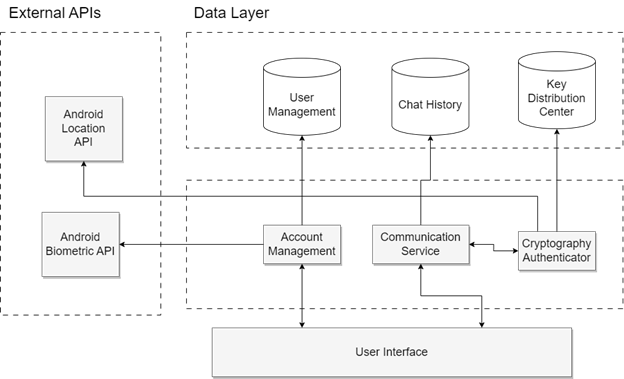
\includegraphics{blockdiagram.png}
% End SubSection

\subsection{Product Functions}
\label{sub:product_functions}
% Begin SubSection
There are 4 main modules that are going to be implemented in VanklComm. These modules are the Communication module, the Account Management module, the Cryptography module, and the Database module. The Communication module will oversee most of the business value of the application, which includes chatting. The Account Management module will deal with creation and deletion of accounts, as well as implementing the company structure and verifying that the agents are authorized. The Cryptography module will deal with message encryption and decryption. The Database module will oversee how the chat logs are stored.

\begin{center}
	\begin{tabular}{| p{4cm} | p{13cm} |}
		\hline
		\textbf{Module}           & \textbf{Function}                   \\
		\hline
		Communication Module      &
		\begin{itemize}
			\item Connect to chat
			      \begin{itemize}
				      \item Allows user to connect to the chat
			      \end{itemize}
			\item Send and receive messages
			      \begin{itemize}
				      \item Allows user to send and receive messages from other users
			      \end{itemize}
			\item[\textcolor{red}{•}] \textcolor{red}{Send and receive files
				\begin{itemize}
					\item Allows user to send and receive files from other users
				\end{itemize}
			\item Receive announcement board posts
			      \begin{itemize}
				      \item Allows user to receive messages from managers through the announcement board
			      \end{itemize}
			      }
			\item Report inappropriate messages
			      \begin{itemize}
				      \item Allows user to report inappropriate messages to admin
			      \end{itemize}
		\end{itemize} \\
		\hline
		Account Management Module &
		\begin{itemize}
			\item Create account
			      \begin{itemize}
				      \item Allows user to create account
			      \end{itemize}
			\item Delete account
			      \begin{itemize}
				      \item Allows user to delete account
			      \end{itemize}
			\item[\textcolor{red}{•}] \textcolor{red}{Create a contact list
				\begin{itemize}
					\item Allows user to have a contact list with their frequently contacted co-workers
				\end{itemize}
			\item Manage Geolocation
			      \begin{itemize}
				      \item Verifies that user is in the correct location
			      \end{itemize}
			      }
			\item Verify agents are authorized
			      \begin{itemize}
				      \item Oversees correct user credentials to allow signing in
				      \item[\textcolor{red}{–}] \textcolor{red}{Verify user using biometrics}
			      \end{itemize}
		\end{itemize}  \\
		\hline
		Cryptography Module       &
		\begin{itemize}
			\item Manage the KDC
			      \begin{itemize}
				      \item Ensures that the KDC works as expected
			      \end{itemize}
			\item Encrypt sent messages
			      \begin{itemize}
				      \item Encrypts the sent messages
			      \end{itemize}
			\item Decrypt received messages
			      \begin{itemize}
				      \item Decrypts the received messages
			      \end{itemize}
		\end{itemize}                                  \\
		\hline
		Database Module           &
		\begin{itemize}
			\item Store chat logs
			      \begin{itemize}
				      \item Stores all chat logs in a secure database
			      \end{itemize}
		\end{itemize}                                   \\
		\hline
	\end{tabular}

	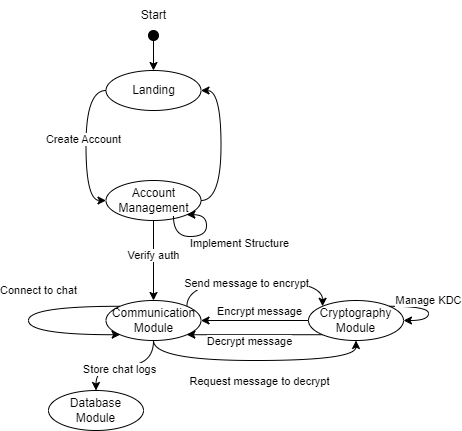
\includegraphics[scale = 0.8]{3A04_D1.png}
\end{center}
% End SubSection

\subsection{User Characteristics}
\label{sub:user_characteristics}
% Begin SubSection
Education Skills: Basic Reading and Writing Skills
\begin{itemize}
	\item Users are expected to have a basic understanding of the language used in the app, to be able to navigate different parts of the app, and to talk and text through the app
	      %	\item Do not state specific requirements, but rather provide the reasons why certain specific requirements are later specified
\end{itemize}
% End SubSection
\label{sub:user_characteristics}
% Begin SubSection
Experience: No specific experience required
\begin{itemize}
	\item Users could be familiar with common messaging applications, but the application will be intuitive and user-friendly for anyone, even those who don't have much experience with messaging applications.
	      %	\item Do not state specific requirements, but rather provide the reasons why certain specific requirements are later specified
\end{itemize}
% End SubSection
% Begin SubSection
Technical Skills: Should be able to use a smartphone
\begin{itemize}
	\item Users should have a basic understanding of how to use a smartphone, download apps and navigate different features of the hardware to be able to use the app and communicate through it.
	      %	\item Do not state specific requirements, but rather provide the reasons why certain specific requirements are later specified
\end{itemize}
% End SubSection
\noindent {\bf Roles}\\
\label{sub:user_characteristics}
% Begin SubSection

Managers
\begin{itemize}
	\item Managers will be able to send announcements through to many employees in a one way communication channel.
	      %	\item Do not state specific requirements, but rather provide the reasons why certain specific requirements are later specified
\end{itemize}
% End SubSection
\label{sub:user_characteristics}
% Begin SubSection
Employee
\begin{itemize}
	\item Basic communication abilities, can message, call, share files, etc. with others. Can not make announcements like managers.
	      %	\item Do not state specific requirements, but rather provide the reasons why certain specific requirements are later specified
\end{itemize}
% End SubSection

\subsection{Constraints}
\label{sub:constraints}
% Begin SubSection
\begin{itemize}
	\item Provide a general description of any constraints that will limit the developer's options
\end{itemize}
% End SubSection

\subsection{Assumptions and Dependencies}
\label{sub:assumptions_and_dependencies}
% Begin SubSection
\begin{itemize}
	\item List any assumptions you made in interpreting what the software being developed is aiming to achieve
	\item List any other assumptions you made that, if it fails to hold, could require you to change the requirements
	      %\item List each of the factors that affect the requirements stated in the SRS
	      %\item These factors are not design constraints on the software but are, rather, any changes to them that can affect the requirements in the SRS
	      \begin{itemize}
		      \item \textbf{Example}: An assumption may be that a specific operating system will be available on the hardware designated for the software product. If, in fact, the operating system is not available, the SRS would then have to change accordingly.
	      \end{itemize}
\end{itemize}
% End SubSection

\subsection{Apportioning of Requirements}
\label{sub:apportioning_of_requirements}
% Begin SubSection
\subsection*{1. Cross-Platform Compatibility:}
The initial version of the secure chat application will be strictly developed for the Android platform. However, we will consider extending support to iOS and other mobile operating systems in later versions. This will allow our application to cater to a wider variety of users.

\subsection*{2. Secure Group Chat Communication:}
The initial version of our application will only provide encrypted one-on-one communication between company employees. Future versions may introduce a group chat feature, which allows multiple users to communicate in a group setting, all the while ensuring a safe and secure platform. This will benefit users by allowing them to efficiently coordinate tasks with many employees, including file transfer, calendar scheduling, and more.

\subsection*{3. Secure Video Conferencing:}
The app’s initial version only considers communication in terms of text-based messages and file sharing between users. However, later versions could support an integration with secure video conferencing systems, allowing users to interact in encrypted video calls for a more immersive experience.
% End SubSection

% End Section
\section{Use Case Diagram}
\label{sec:use_case_diagram}
% Begin Section
\begin{itemize}
	\item Provide the use case diagram for the system being developed.
	\item You do not need to provide the textual description of any of the use cases here (these will be specified under "Highlights of Functional Requirements").
	      %	\item Provide \emph{one} use case diagram for the most important Business Event.
	      %	\item The text of all use cases will be specified under "Highlights of Functional Requirements"
\end{itemize}
%In this section, select the most important Business Event that your system responds to and give its use case diagram.  Only one use case diagram is needed.  Give a brief textual description of the use case without repeating what is in the scenarios of the corresponding Business Event.

%
%
%
%This section should provide a use case diagram for your application. 
%\begin{enumerate}[a)]
%	\item Each use case appearing in the diagram should be accompanied by a text description. 
%\end{enumerate}
%% End Section

\section{Highlights of Functional Requirements}
\label{sec:functional_requirements}
% Begin Section

\noindent {\bf Main Business Events:} List out all the main business events you are presenting. If you sub-divided into smaller ones, you don't need to include the smaller ones in this list.\\

\begin{itemize}
	\item BE1 Secure Communication
	\item BE2 Chat History Log
	\item[\textcolor{red}{\textbullet}] \textcolor{red}{BE3 Contact Book}
	\item BE4 Secure File Sharing
	\item[\textcolor{red}{\textbullet}] \textcolor{red}{BE5 Broadcasting Channel}
	\item BE6 User Registration
	\item BE7 Authentication Protocol
	\item BE8 Key Updates
	\item[\textcolor{red}{\textbullet}] \textcolor{red}{BE9 Biometric Authentication}
	\item[\textcolor{red}{\textbullet}] \textcolor{red}{BE10 Geolocation}
	
\end{itemize}

\noindent {\bf Viewpoints:} List out all the viewpoints you will be considering.\\

\begin{itemize}
	\item VP1 User
	\item 	VP2 Tech Support/IT
	\item 	VP3 KDC Administrator
	\item 	VP4 Security Auditors/Cybersecurity
	\item 	VP5 Legal Department
	\item 	VP6 Board of Directors
	
	
\end{itemize}

\noindent {\bf Interpretation:} Specify any liberties you took in interpreting business events, if necessary.\\

\section*{Business Events:}
\subsection*{1BE. Secure Communication \#1}
\subsubsection*{Precondition:} The secure chat application has already been installed on an Android device, and the user has an account.
\subsubsection*{1VP. User \#1}
\textbf{Main Success Scenario:}
\begin{enumerate}
    \item The user logs into the VANKL secure chat application.
    \item The system authenticates the user.
    \item Once authenticated, the user may engage in various tasks, including secure communication, accessing the chat’s history log, utilizing the contact book, sharing files securely, and receiving broadcasts from higher authority.
\end{enumerate}
\textbf{Secondary Scenarios:}
\begin{enumerate}
    \item[\textbf{2i.}] The system fails to authenticate the user.
    \begin{enumerate}
        \item[\textbf{2i.1}] The system will prompt the user to retry for authentication.
        \item[\textbf{2i.2}] If the issue persists, then the user will be redirected to contact tech support.
    \end{enumerate}
    \item[\textbf{3i.}] The user experiences delays when trying to access the chat’s history log, due to server overload issues.
    \begin{enumerate}
        \item[\textbf{3i.1}] The system provides a display message to inform the user of this delay and apologizes for the inconvenience.
        \item[\textbf{3i.2}] The system will continuously attempt to alleviate the increased demand, by utilizing backup servers, caching, and load balancing.
    \end{enumerate}
\end{enumerate}
\subsubsection*{2VP. Tech Support/IT \#2}
\begin{enumerate}
    \item[\textbf{2i.}] The system fails to authenticate Tech Support/IT.
    \item[\textbf{3i.}] Tech Support/IT faces challenges during debugging and troubleshooting, due to an unexpected server outage.
\end{enumerate}
\subsubsection*{3VP. KDC Administrator \#3}
\textbf{N/A}
\subsubsection*{4VP. Security Auditors/Cybersecurity \#4}
\begin{enumerate}
    \item[\textbf{2i.}] The system fails to authenticate the Security Auditors/Cybersecurity.
    \item[\textbf{3i.}] The Security Auditors/Cybersecurity encounter issues while accessing specific logs, due to a temporary system glitch.
\end{enumerate}
\subsubsection*{5VP. Legal Department \#5}
\textbf{N/A}
\subsubsection*{6VP. Board of Directors \#6}
\begin{enumerate}
    \item[\textbf{2i.}] The system fails to authenticate the Board of Directors.
    \item[\textbf{3i.}] The Board of Directors encounter delays while sending a one-way message in the broadcasting channel, due to server overload.
\end{enumerate}
\textbf{Global Scenario:}
\subsubsection*{Precondition:} The secure chat application has already been installed on an Android device, the user has an account, and all necessary configurations have been made.\newline\newline
\textbf{Main Success Scenario:}
\begin{enumerate}
    \item The user, Tech Support/IT, Security Auditors/Cybersecurity, Legal Department, and the Board of Directors all log into the VANKL secure chat application (not necessarily simultaneously).
    \item The system authenticates each entity successfully.
    \item Each entity performs their respective tasks and actions within the application.
\end{enumerate}
\textbf{Secondary Scenarios:}
\begin{enumerate}
    \item[\textbf{2i.}] The system fails to authenticate any entity.
    \begin{enumerate}
        \item[\textbf{2i.1}] The system will prompt that entity to retry for authentication.
        \item[\textbf{2i.2}] If the issue persists, then that entity will be redirected to contact their respective support department (not necessarily Tech Support/IT).
    \end{enumerate}
    \item[\textbf{3i.}] An entity faces issues related to the various functionalities of the application, due to server problems.
    \begin{enumerate}
        \item[\textbf{3i.1}] The system provides a global display message to acknowledge the issue(s), and assures the entity(s) that Tech Support/IT is working on a resolution.
    \end{enumerate}
\end{enumerate}

\section*{2BE. Chat History Log \#2}
\subsubsection*{Precondition:} The secure chat application has already been installed on an Android device, and the user has an account.
\subsubsection*{1VP. User \#1}
\textbf{Main Success Scenario:}
\begin{enumerate}
    \item The user logs into the VANKL secure chat application.
    \item The system authenticates the user.
    \item Once authenticated, the user can access their chat’s history log.
    \item The system displays specific identifiers, date, time, and an up-to-date chat transcript for each conversation.
\end{enumerate}
\textbf{Secondary Scenarios:}
\begin{enumerate}
    \item[\textbf{2i.}] The system fails to authenticate the user.
    \begin{enumerate}
        \item[\textbf{2i.1}] The system will prompt the user to retry for authentication.
        \item[\textbf{2i.2}] If the issue persists, then the user will be redirected to contact tech support.
    \end{enumerate}
    \item[\textbf{3i.}] The user experiences delays when trying to access the chat’s history log, due to server overload issues.
    \begin{enumerate}
        \item[\textbf{3i.1}] The system provides a display message to inform the user of this delay and apologizes for the inconvenience.
        \item[\textbf{3i.2}] The system will continuously attempt to alleviate the increased demand, by utilizing backup servers, caching, and load balancing.
    \end{enumerate}
    \item[\textbf{4i.}] While viewing a specific conversation, the system experiences a temporary glitch, which results in missing or incomplete messages.
    \begin{enumerate}
        \item[\textbf{4i.1}] The system provides a display message to inform the user of this issue, and apologizes for the inconvenience.
        \item[\textbf{4i.2}] The system then advises the user to refresh the chat log or contact Tech Support/IT, if the problem still persists.
    \end{enumerate}
\end{enumerate}
\subsubsection*{2VP. Tech Support/IT \#2}
\textbf{N/A}
\subsubsection*{3VP. KDC Administrator \#3}
\textbf{N/A}
\subsubsection*{4VP. Security Auditors/Cybersecurity \#4}
\textbf{N/A}
\subsubsection*{5VP. Legal Department \#5}
\textbf{N/A}
\subsubsection*{6VP. Board of Directors \#6}
\textbf{N/A}\newline\newline
\textbf{Global Scenario:}
\subsubsection*{Precondition:} The secure chat application has already been installed on an Android device, the user has an account, and all necessary configurations have been made.\newline\newline
\textbf{Main Success Scenario:}
\begin{enumerate}
    \item The user, Tech Support/IT, Security Auditors/Cybersecurity, Legal Department, and the Board of Directors all log into the VANKL secure chat application (not necessarily simultaneously).
    \item The system authenticates each entity successfully.
    \item Each entity accesses their respective chat history log that has accurate and up-to-date conversation records.
\end{enumerate}
\textbf{Secondary Scenarios:}
\begin{enumerate}
    \item[\textbf{2i.}] The system fails to authenticate any entity.
    \begin{enumerate}
        \item[\textbf{2i.1}] The system will prompt that entity to retry for authentication.
        \item[\textbf{2i.2}] If the issue persists, then that entity will be redirected to contact their respective support department (not necessarily Tech Support/IT).
    \end{enumerate}
    \item[\textbf{3i.}] An entity faces delays in accessing specific chat history logs, due to server problems.
    \begin{enumerate}
        \item[\textbf{3i.1}] The system provides a global display message to acknowledge the issue(s), and assures the entity(s) that Tech Support/IT is working on a resolution.
    \end{enumerate}
    \item[\textbf{4i.}] An entity faces system glitches, resulting in missing or incomplete messages while viewing conversations.
    \begin{enumerate}
        \item[\textbf{4i.1}] The system provides an error message and advises the entity(s) to report this issue to management (Board of Directors), who will in turn contact Tech Support/IT for investigating this issue.
    \end{enumerate}
\end{enumerate}


\section*{\textcolor{red}{3BE. Contact Book \#3}}
\subsubsection*{Precondition:} The secure chat application has already been installed on an Android device, and the user has an account.
\subsubsection*{1VP. User \#1}
\textbf{Main Success Scenario:}
\begin{enumerate}
    \item The user logs into the VANKL secure chat application.
    \item The system authenticates the user.
    \item Once authenticated, the user can access their contact book.
    \item The system provides saved agents’ contact information for easier communication access.
    \item The user can easily add, edit, and/or delete contacts as required.
\end{enumerate}
\textbf{Secondary Scenarios:}
\begin{enumerate}
    \item[\textbf{2i.}] The system fails to authenticate the user.
    \begin{enumerate}
        \item[\textbf{2i.1}] The system will prompt the user to retry for authentication.
        \item[\textbf{2i.2}] If the issue persists, then the user will be redirected to contact tech support.
    \end{enumerate}
    \item[\textbf{3i.}] The user experiences delays when trying to access their contact book, due to server overload issues.
    \begin{enumerate}
        \item[\textbf{3i.1}] The system provides a display message to inform the user of this delay, and apologizes for the inconvenience.
        \item[\textbf{3i.2}] The system will continuously attempt to alleviate the increased demand, by utilizing backup servers, caching, and load balancing.
    \end{enumerate}
    \item[\textbf{4i.}] When searching for an employee’s contact, the system experiences a temporary glitch, which leads to missing contact information.
    \begin{enumerate}
        \item[\textbf{4i.1}] The system provides a display message to inform the user of this error, and apologizes for the inconvenience.
        \item[\textbf{4i.2}] The system advises the user to refresh the contact book or contact Tech Support/IT, if the issue still persists.
    \end{enumerate}
    \item[\textbf{5i.}] When accessing the contact book to add, edit, and/or delete contacts, the system faces a navigation malfunction.
    \begin{enumerate}
        \item[\textbf{5i.1}] When the user attempts to access the contact book feature, the system runs into a malfunction with the navigation subsystem.
        \item[\textbf{5i.2}] The system provides an error message to the user apologizing for the inconvenience and logs an incident report for the tech team to assess and resolve.
    \end{enumerate}
\end{enumerate}
\subsubsection*{2VP. Tech Support/IT \#2}
\textbf{N/A}
\subsubsection*{3VP. KDC Administrator \#3}
\textbf{N/A}
\subsubsection*{4VP. Security Auditors/Cybersecurity \#4}
\textbf{N/A}
\subsubsection*{5VP. Legal Department \#5}
\textbf{N/A}
\subsubsection*{6VP. Board of Directors \#6}
\textbf{N/A}\newline\newline
\textbf{Global Scenario:}
\subsubsection*{Precondition:} The secure chat application has already been installed on an Android device, the user has an account, and all necessary configurations have been made.\newline\newline
\textbf{Main Success Scenario:}
\begin{enumerate}
    \item The user, Tech Support/IT, Security Auditors/Cybersecurity, Legal Department, and the Board of Directors all log into the VANKL secure chat application (not necessarily simultaneously).
    \item The system authenticates each entity successfully.
    \item Only the users can access the contact book and view their saved agents’ information for easier communication access.
\end{enumerate}
\textbf{Secondary Scenarios:}
\begin{enumerate}
    \item[\textbf{2i.}] The system fails to authenticate any entity.
    \begin{enumerate}
        \item[\textbf{2i.1}] The system will prompt that entity to retry for authentication.
        \item[\textbf{2i.2}] If the issue persists, then that entity will be redirected to contact their respective support department (not necessarily Tech Support/IT).
    \end{enumerate}
    \item[\textbf{3i.}] A user faces issues when trying to open their contact book, such as accessing delays or missing/incomplete contact information.
    \begin{enumerate}
        \item[\textbf{3i.1}] The system provides a display message to acknowledge that Tech Support/IT is working on a resolution.
        \item[\textbf{3i.2}] The system advises the user to refresh the contact book or access it at a later time.
    \end{enumerate}
\end{enumerate}

\section*{4BE. Secure File Sharing \#4}
\subsubsection*{Precondition:} The secure chat application has already been installed on an Android device, and the user has an account.
\subsubsection*{1VP. User \#1}
\textbf{Main Success Scenario:}
\begin{enumerate}
    \item The user logs into the VANKL secure chat application.
    \item The system authenticates the user.
    \item Once authenticated, the user can initiate secure file sharing.
    \item The system will encrypt the file and facilitate secure transmission.
    \item The file recipient will then decrypt and access the shared file.
\end{enumerate}
\textbf{Secondary Scenarios:}
\begin{enumerate}
    \item[\textbf{2i.}] The system fails to authenticate the user.
    \begin{enumerate}
        \item[\textbf{2i.1}] The system will prompt the user to retry for authentication.
        \item[\textbf{2i.2}] If the issue persists, then the user will be redirected to contact tech support.
    \end{enumerate}
    \item[\textbf{3i.}] The user experiences delays when trying to initiate secure file transfer, due to server overload issues.
    \begin{enumerate}
        \item[\textbf{3i.1}] The system provides a display message to inform the user of this delay, and apologizes for the inconvenience.
        \item[\textbf{3i.2}] The system will continuously attempt to alleviate the increased demand, by utilizing backup servers, caching, and load balancing.
    \end{enumerate}
    \item[\textbf{4i.}] When encrypting the file, the system experiences a temporary glitch, which leads to a delay in the transmission process.
    \begin{enumerate}
        \item[\textbf{4i.1}] The system provides a display message to inform the user of this error, and apologizes for the inconvenience.
        \item[\textbf{4i.2}] The system advises the user to retry file sharing or contact Tech Support/IT, if the issue still persists.
    \end{enumerate}
\end{enumerate}
\subsubsection*{2VP. Tech Support/IT \#2}
\textbf{N/A}
\subsubsection*{3VP. KDC Administrator \#3}
\textbf{N/A}
\subsubsection*{4VP. Security Auditors/Cybersecurity \#4}
\textbf{N/A}
\subsubsection*{5VP. Legal Department \#5}
\textbf{N/A}
\subsubsection*{6VP. Board of Directors \#6}
\textbf{N/A}\newline\newline
\textbf{Global Scenario:}
\subsubsection*{Precondition:} The secure chat application has already been installed on an Android device, the user has an account, and all necessary configurations have been made.\newline\newline
\textbf{Main Success Scenario:}
\begin{enumerate}
    \item The user, Tech Support/IT, Security Auditors/Cybersecurity, Legal Department, and the Board of Directors all log into the VANKL secure chat application (not necessarily simultaneously).
    \item The system authenticates each entity successfully.
    \item Only the users can initiate secure file transfer between the employees of the company.
\end{enumerate}
\textbf{Secondary Scenarios:}
\begin{enumerate}
    \item[\textbf{2i.}] The system fails to authenticate any entity.
    \begin{enumerate}
        \item[\textbf{2i.1}] The system will prompt that entity to retry for authentication.
        \item[\textbf{2i.2}] If the issue persists, then that entity will be redirected to contact their respective support department (not necessarily Tech Support/IT).
    \end{enumerate}
    \item[\textbf{3i.}] A user faces delays in the secure file sharing process, due to server issues.
    \begin{enumerate}
        \item[\textbf{3i.1}] The system provides a display message to acknowledge that Tech Support/IT is working on a resolution.
        \item[\textbf{3i.2}] The system advises the user to retry the file transfer or try again at a later time.
    \end{enumerate}
    \item[\textbf{4i.}] The system faces temporary glitches resulting in missing/incomplete file transfer.
    \begin{enumerate}
        \item[\textbf{4i.1}] The system provides a display message to acknowledge that Tech Support/IT is working on a resolution.
        \item[\textbf{4i.2}] The system advises the user to retry the file transfer when the glitches have been fixed at a later date.
    \end{enumerate}
\end{enumerate}

\section*{\textcolor{red}{5BE. Broadcasting Channel \#5}}
\subsubsection*{Precondition:} The secure chat application has already been installed on an Android device, and the user has an account.
\subsubsection*{1VP. User \#1}
\textbf{Main Success Scenario:}
\begin{enumerate}
    \item The user logs into the VANKL secure chat application.
    \item The system authenticates the user.
    \item Once authenticated, the user can access the one-way broadcasting channel feature.
    \item The system allows users to view the broadcasted announcements sent out by their superiors (i.e. Board of Directors).
\end{enumerate}
\textbf{Secondary Scenarios:}
\begin{enumerate}
    \item[\textbf{2i.}] The system fails to authenticate the user.
    \begin{enumerate}
        \item[\textbf{2i.1}] The system will prompt the user to retry for authentication.
        \item[\textbf{2i.2}] If the issue persists, then the user will be redirected to contact tech support.
    \end{enumerate}
    \item[\textbf{3i.}] The user experiences delays when trying to access the broadcasting channel, due to server overload issues.
    \begin{enumerate}
        \item[\textbf{3i.1}] The system provides a display message to inform the user of this delay, and apologizes for the inconvenience.
        \item[\textbf{3i.2}] The system will continuously attempt to alleviate the increased demand, by utilizing backup servers, caching, and load balancing.
    \end{enumerate}
    \item[\textbf{4i.}] The system experiences a temporary glitch, which leads to missing one-way messages in the broadcasting channel.
    \begin{enumerate}
        \item[\textbf{4i.1}] The system provides a display message to inform the user of this issue, and apologizes for the inconvenience.
        \item[\textbf{4i.2}] The system advises the user to report this issue to Tech Support/IT.
    \end{enumerate}
\end{enumerate}
\subsubsection*{2VP. Tech Support/IT \#2}
\textbf{N/A}
\subsubsection*{3VP. KDC Administrator \#3}
\textbf{N/A}
\subsubsection*{4VP. Security Auditors/Cybersecurity \#4}
\textbf{N/A}
\subsubsection*{5VP. Legal Department \#5}
\textbf{N/A}
\subsubsection*{6VP. Board of Directors \#6}
\begin{enumerate}
    \item[\textbf{2i.}] The system fails to authenticate a Board of Directors member.
    \item[\textbf{3i.}] The Board of Directors member experiences delays when trying to access the broadcasting channel, due to server overload issues.
    \item[\textbf{4i.}] The system experiences a temporary glitch, which leads to missing one-way messages (that a member has sent) in the broadcasting channel.
\end{enumerate}
\textbf{Global Scenario:}
\subsubsection*{Precondition:} The secure chat application has already been installed on an Android device, the user has an account, and all necessary configurations have been made.\newline\newline
\textbf{Main Success Scenario:}
\begin{enumerate}
    \item The user, Tech Support/IT, Security Auditors/Cybersecurity, Legal Department, and the Board of Directors all log into the VANKL secure chat application (not necessarily simultaneously).
    \item The system authenticates each entity successfully.
    \item Only the users and the Board of Directors can utilize the broadcasting channel feature, where users (i.e. employees) can view one-way messages and board members can send one-way messages.
\end{enumerate}
\textbf{Secondary Scenarios:}
\begin{enumerate}
    \item[\textbf{2i.}] The system fails to authenticate any entity.
    \begin{enumerate}
        \item[\textbf{2i.1}] The system will prompt that entity to retry for authentication.
        \item[\textbf{2i.2}] If the issue persists, then that entity will be redirected to contact their respective support department (not necessarily Tech Support/IT).
    \end{enumerate}
    \item[\textbf{3i.}] An entity faces delays in accessing the broadcasting channel, due to server issues.
    \begin{enumerate}
        \item[\textbf{3i.1}] The system provides a display message to acknowledge that Tech Support/IT is working on a resolution.
        \item[\textbf{3i.2}] The system advises the entity(s) to refresh the broadcasting channel or try again at a later time.
    \end{enumerate}
    \item[\textbf{4i.}] The system faces temporary glitches resulting in missing/incomplete one-way messages in the broadcasting channel.
    \begin{enumerate}
        \item[\textbf{4i.1}] The system provides a display message to acknowledge that Tech Support/IT is working on a resolution.
        \item[\textbf{4i.2}] The system advises the entity(s) to access the broadcasting channel when the glitches have been fixed at a later date.
    \end{enumerate}
\end{enumerate}

\section*{6BE. User Registration \#6}
\subsubsection*{Precondition:} 
\begin{itemize}
	\item User does not have an account
	\item User was granted access to company issued device/email
	\item User is connected to company WIFI
	\item The KDC server is operational
\end{itemize}
\subsubsection*{1VP. User \#1}
\textbf{Main Success Scenario:}
\begin{enumerate}
    \item User gains access to make an account
	\item User initiates sign in
	\item User inputs information
	\item User is provided key from KDC
	\item User is prompted with success message
\end{enumerate}
\textbf{Secondary Scenarios:}
\begin{enumerate}
    \item[\textbf{2i.}] User inputs incorrect information
    \begin{enumerate}
		\item[\textbf{2i.1}] User submits incorrect information
        \item[\textbf{2i.2}] Prompts user to recheck information and resubmit
    \end{enumerate}
\end{enumerate}
\subsubsection*{2VP. Tech Support/IT \#2}
\begin{enumerate}
    \item[\textbf{1i.}] IT provides the app with authorization for user's information and provided email	
\end{enumerate}
\subsubsection*{3VP. KDC Administrator \#3}
\begin{enumerate}
    \item[\textbf{4i.}] KDC provides key
    \begin{enumerate}
        \item[\textbf{4i.1}] KDC checks users authorization status
        \item[\textbf{4i.2}] KDC generates encryption key
    \end{enumerate}
    \item[\textbf{4i.}] User inputted incorrect information
    \begin{enumerate}
        \item[\textbf{4i.1}] KDC checks user authorization status
        \item[\textbf{4i.2}] Denies access and does not generate key
    \end{enumerate}
\end{enumerate}
\subsubsection*{4VP. Security Auditors/Cybersecurity \#4}
\textbf{N/A}
\subsubsection*{5VP. Legal Department \#5}
\textbf{N/A}
\subsubsection*{6VP. Board of Directors \#6}
\textbf{N/A}\\

\noindent \textbf{Global Scenario:}
\subsubsection*{Precondition:} 
\begin{itemize}
	\item User does not have an account
	\item User was granted access to company issued device/email
	\item User is connected to company WIFI
	\item The KDC server is operational
\end{itemize}
\textbf{Main Success Scenario:}
\begin{enumerate}
	\item User gains access to make an account
	\item User initiates sign in
	\item User inputs information
	\item User is provided key from KDC
	\item User is prompted with success message
\end{enumerate}
\textbf{Secondary Scenarios:}
\begin{enumerate}
    \item[\textbf{2i.}] User inputs incorrect information
    \begin{enumerate}
		\item[\textbf{2i.1}] User submits incorrect information
        \item[\textbf{2i.2}] Prompts user to recheck information and resubmit
    \end{enumerate}
\end{enumerate}

\section*{7BE. Authentication Protocol \#7}
\subsubsection*{Precondition:} 
\begin{itemize}
    \item User attempts to access the chat application
    \item Initiates authentication process
\end{itemize}
\subsubsection*{1VP. User \#1}
\textbf{Main Success Scenario:}
\begin{enumerate}
    \item The user opens the chat application
    \item The user provides their username and password to sign in to the chat application
    \item The application authenticates the user's credentials
    \item Upon successful authentication, the user gains access to the application's features
\end{enumerate}
\textbf{Secondary Success Scenario:}
\begin{enumerate}
    \item[\textbf{2i.}] User inputs incorrect information
    \begin{enumerate}
        \item[\textbf{2i.1}] Prompted to re-enter information
    \end{enumerate}
\end{enumerate}
\subsubsection*{2VP. Tech Support/IT \#2}
\begin{enumerate}
    \item[\textbf{2i.}] User has too many failed attempts to authenticate
    \begin{enumerate}
        \item[\textbf{2i.1}] IT support is notified of the failed attempts
        \item[\textbf{2i.2}] IT support will contact the user to assist with the authentication process
        \item[\textbf{2i.3}] IT support will reset the user's password if necessary
    \end{enumerate}
\end{enumerate}
\subsubsection*{3VP. KDC Administrator \#3}
\textbf{N/A}
\subsubsection*{4VP. Security Auditors/Cybersecurity \#4}
\textbf{N/A}
\subsubsection*{5VP. Legal Department \#5}
\textbf{N/A}
\subsubsection*{6VP. Board of Directors \#6}
\textbf{N/A}\\

\noindent \textbf{Global Scenario:}
\subsubsection*{Precondition:} 
\begin{itemize}
    \item User attempts to access the chat application
    \item Initiates authentication process
\end{itemize}
\textbf{Main Success Scenario:}
\begin{enumerate}
    \item User opens the chat application
    \item User provides their username and password
    \item The application authenticates the user's credentials
    \item Upon successful authentication, the user gains access to the application's features
\end{enumerate}
\textbf{Secondary Success Scenario:}
\begin{enumerate}
    \item[\textbf{2i.}] User inputs incorrect information
    \begin{enumerate}
        \item[\textbf{2i.1}] Prompted to re-enter information
    \end{enumerate}
\end{enumerate}

\section*{8BE. Key Update \#8}
\subsubsection*{Precondition:} 
\begin{itemize}
    \item The KDC has new keys to distribute for secure communication.
\end{itemize}
\subsubsection*{1VP. User}
\textbf{Main Success Scenario:}
\begin{enumerate}
    \item KDC sends new key updates to user’s device
    \item User receives a notification about the availability of new keys.
    \item User's device automatically updates the keys without requiring manual intervention
    \item User continues to use the secure chat application with updated keys
\end{enumerate}
\textbf{Secondary Success Scenario:}
\begin{enumerate}
    \item[\textbf{2i.}] User misses notification/update because they were disconnected
    \begin{enumerate}
        \item[\textbf{2i.1}] User can manually hit update button and update keys
    \end{enumerate}
\end{enumerate}
\subsubsection*{2VP. Tech Support/IT \#2}
\textbf{N/A}
\subsubsection*{3VP. KDC Administrator \#3}
\begin{enumerate}
    \item[\textbf{1i.}] KDC generates new keys and pushes notifications for key updates
    \begin{enumerate}
    	\item[\textbf{1i.1}] KDC sends new key updates to user’s device
    	\item[\textbf{1i.2}] KDC sends a notification about the availability of new keys
	\end{enumerate}	
\end{enumerate}
\subsubsection*{4VP. Security Auditors/Cybersecurity \#4}
\begin{enumerate}
    \item[\textbf{1i.}] Security Auditors/Cybersecurity monitors the key update process
    \begin{enumerate}
		\item[\textbf{1i.1}] Security Auditors/Cybersecurity checks the integrity of the new keys
		\item[\textbf{1i.2}] Security Auditors/Cybersecurity ensure the new keys are distributed securely 
	\end{enumerate}
\end{enumerate}
\subsubsection*{5VP. Legal Department \#5}
\textbf{N/A}
\subsubsection*{6VP. Board of Directors \#6}
\textbf{N/A}\\

\noindent \textbf{Global Scenario:}
\subsubsection*{Precondition:} 
\begin{itemize}
    \item The KDC has new keys to distribute for secure communication.
\end{itemize}
\textbf{Main Success Scenario:}
\begin{enumerate}
    \item KDC sends new key updates to user’s device
    \item User receives a notification about the availability of new keys.
    \item User's device automatically updates the keys without requiring manual intervention
    \item User continues to use the secure chat application with updated keys
\end{enumerate}
\textbf{Secondary Success Scenario:}
\begin{enumerate}
    \item[\textbf{2i.}] User misses notification/update because they were disconnected
    \begin{enumerate}
        \item[\textbf{2i.1}] User can manually hit update button and update keys
    \end{enumerate}
\end{enumerate}

\section*{\textcolor{red}{9BE. Biometric Authentication \#9}}
\subsubsection*{Preconditions:} 
\begin{itemize}
    \item User has biometric authentication enabled
    \item Device has methods of biometric authentication built-in
    \item Chat application supports biometric authentication
\end{itemize}
\subsubsection*{1VP. User}
\textbf{Main Success Scenario:}
\begin{enumerate}
    \item User opens the app
    \item The app prompts the user for biometric authentication (ex. fingerprint, facial recognition)
    \item User provides biometric data
    \item The app verifies the biometric data and grants access to the app upon successful authentication
\end{enumerate}
\textbf{Secondary Success Scenario:}
\begin{enumerate}
    \item[\textbf{4i.}] Biometric data fails
    \begin{enumerate}
        \item[\textbf{4i.1}] Prompts user to enter password
        \item[\textbf{4i.2}] Grants access to app with correct password
    \end{enumerate}
\end{enumerate}
\subsubsection*{2VP. Tech Support/IT}
\textbf{N/A}
\subsubsection*{3VP. KDC Administrator}
\textbf{N/A}
\subsubsection*{4VP. Security Auditors/Cybersecurity}
\begin{enumerate}
    \item[\textbf{4i.}] Security Auditors/Cybersecurity ensure biometric data and authentication is secure
    \begin{enumerate}
        \item[\textbf{4i.1}] Biometric data is provided by the user
        \item[\textbf{4i.2}] Biometric data is encrypted and stored securely on the device
    \end{enumerate}
\end{enumerate}
\subsubsection*{5VP. Legal Department}
\textbf{N/A}
\subsubsection*{6VP. Board of Directors}
\textbf{N/A}

\subsection*{Global Scenario:}
\subsubsection*{Preconditions:} 
\begin{itemize}
    \item User has biometric authentication enabled
    \item Device has methods of biometric authentication built-in
    \item Chat application supports biometric authentication
\end{itemize}
\textbf{Main Success Scenario:}
\begin{enumerate}
    \item User opens the app
    \item The app prompts the user for biometric authentication (ex. fingerprint, facial recognition)
    \item User provides biometric data
    \item The app verifies the biometric data and grants access to the app upon successful authentication
\end{enumerate}
\textbf{Secondary Success Scenario:}
\begin{enumerate}
    \item[\textbf{4i.}] Biometric data fails
    \begin{enumerate}
        \item[\textbf{4i.1}] Prompts user to enter password
        \item[\textbf{4i.2}] Grants access to app with correct password
    \end{enumerate}
\end{enumerate}


\section*{\textcolor{red}{10BE. Geolocation \#10}}
\subsubsection*{Preconditions:} 
\begin{itemize}
    \item The app is installed on the user's device
    \item The device has location services enabled
    \item The company defines specific areas where access to the application is allowed
\end{itemize}
\subsubsection*{1VP. User}
\textbf{Main Success Scenario:}
\begin{enumerate}
    \item User launches the app
    \item The app detects the user's location using geolocation services
    \item If the user is within the designated area, access to the application is granted
    \item User can use the application as usual
\end{enumerate}
\textbf{Secondary Success Scenario:}
\begin{enumerate}
    \item[\textbf{3i.}] User is outside the designated area
    \begin{enumerate}
        \item[\textbf{3i.1}] They are notified that they are outside the designated area
        \item[\textbf{3i.2}] Access to the application is restricted
    \end{enumerate}
\end{enumerate}
\subsubsection*{2VP. Tech Support/IT}
\textbf{N/A}
\subsubsection*{3VP. KDC Administrator}
\textbf{N/A}
\subsubsection*{4VP. Security Auditors/Cybersecurity}
\begin{enumerate}
    \item[\textbf{2i.}] The app detects the users location
    \begin{enumerate}
        \item[\textbf{2i.1}] The application securely stores the user's location data and checks if the user is within the designated area, locally, on the device
    \end{enumerate}
\end{enumerate}
\subsubsection*{5VP. Legal Department}
\textbf{N/A}
\subsubsection*{6VP. Board of Directors}
\textbf{N/A}\\

\noindent \textbf{Global Scenario:}
\subsubsection*{Preconditions:} 
\begin{itemize}
    \item The app is installed on the user's device
    \item The device has location services enabled
    \item The company defines specific areas where access to the application is allowed
\end{itemize}
\textbf{Main Success Scenario:}
\begin{enumerate}
    \item User launches the app
    \item The app detects the user's location using geolocation services
    \item If the user is within the designated area, access to the application is granted
    \item User can use the application as usual
\end{enumerate}
\textbf{Secondary Success Scenario:}
\begin{enumerate}
    \item[\textbf{3i.}] User is outside the designated area
    \begin{enumerate}
        \item[\textbf{3i.1}] They are notified that they are outside the designated area
        \item[\textbf{3i.2}] Access to the application is restricted
    \end{enumerate}
\end{enumerate}



%	Below, we organize by Business Event.
%	\begin{enumerate}[{BE}1.]
%		\item Business Event name
%		\begin{enumerate}[{VP1}.1]
%			\item Viewpoint name \newline
%			\noindent\fbox{%
%				\parbox{0.5\textwidth}{%
%					\begin{itemize}
%						\item {\bf $S_{1}$:} Initial response of the system to the Business Event
%						\item {\bf $E_{1}$:}  Reaction of the environment to $S_{1}$
%						\item {\bf $S_{2}$:}  Response of the system to $E_{1}$
%						\item {\bf $E_{2}$:}  Reaction of the environment to $S_{2}$
%						\item[] $\cdots$
%						\item {\bf $S_{n}$:}  Response of the system to $E_{(n-1)}$
%						\item {\bf $E_{n}$:}  Reaction of the environment to $E_{(n-1)}$
%						\item {\bf $S_{(n+1)}$:} Final response of the system concluding its function regarding the Business Event
%					\end{itemize}
%				}%
%			}
%			\item Viewpoint name\newline
%			\noindent\fbox{%
%				\parbox{0.5\textwidth}{%
%					\begin{itemize}
%						\item {\bf $S_{1}$:} Initial response of the system to the Business Event
%						\item {\bf $E_{1}$:}  Reaction of the environment to $S_{1}$
%						\item {\bf $S_{2}$:}  Response of the system to $E_{1}$
%						\item {\bf $E_{2}$:}  Reaction of the environment to $S_{2}$
%						\item[] $\cdots$
%						\item {\bf $S_{k}$:}  Response of the system to $E_{(k-1)}$
%						\item {\bf $E_{k}$:}  Reaction of the environment to $E_{(k-1)}$
%						\item {\bf $S_{(k+1)}$:} Final response of the system concluding its function regarding the Business Event
%					\end{itemize}
%				}%
%			}
%			\item \dots
%			\item \dots
%			\item \dots
%			\item[\dots]
%		\end{enumerate}	
%		\item[] {\bf Global Scenario of {\it Business Event Name}:} It is the scenario corresponding to the integration of all the above scenarios from the different Viewpoints of the Business Event BE1.\newline
%		\noindent\fbox{%
%			\parbox{0.5\textwidth}{%
%				\begin{itemize}
%					\item {\bf $S_{1}$:} Initial response of the system to the Business Event
%					\item {\bf $E_{1}$:}  Reaction of the environment to $S_{1}$
%					\item {\bf $S_{2}$:}  Response of the system to $E_{1}$
%					\item {\bf $E_{2}$:}  Reaction of the environment to $S_{2}$
%					\item[] $\cdots$
%					\item {\bf $S_{m}$:}  Response of the system to $E_{(m-1)}$
%					\item {\bf $E_{m}$:}  Reaction of the environment to $E_{(m-1)}$
%					\item {\bf $S_{(m+1)}$:} Final response of the system concluding its function regarding the Business Event
%				\end{itemize}
%			}%
%		}	
%		%\end{enumerate}
%		\item Business Event name
%		\begin{enumerate}[{VP1}.1]
%			\item Viewpoint name \newline
%			\noindent\fbox{%
%				\parbox{0.5\textwidth}{%
%					\begin{itemize}
%						\item {\bf $S_{1}$:} Initial response of the system to the Business Event
%						\item {\bf $E_{1}$:}  Reaction of the environment to $S_{1}$
%						\item {\bf $S_{2}$:}  Response of the system to $E_{1}$
%						\item {\bf $E_{2}$:}  Reaction of the environment to $S_{2}$
%						\item[] $\cdots$
%						\item {\bf $S_{n'}$:}  Response of the system to $E_{(n'-1)}$
%						\item {\bf $E_{n'}$:}  Reaction of the environment to $E_{(n'-1)}$
%						\item {\bf $S_{(n'+1)}$:} Final response of the system concluding its function regarding the Business Event
%					\end{itemize}
%				}%
%			}
%			\item Viewpoint name\newline
%			\noindent\fbox{%
%				\parbox{0.5\textwidth}{%
%					\begin{itemize}
%						\item {\bf $S_{1}$:} Initial response of the system to the Business Event
%						\item {\bf $E_{1}$:}  Reaction of the environment to $S_{1}$
%						\item {\bf $S_{2}$:}  Response of the system to $E_{1}$
%						\item {\bf $E_{2}$:}  Reaction of the environment to $S_{2}$
%						\item[] $\cdots$
%						\item {\bf $S_{k'}$:}  Response of the system to $E_{(k'-1)}$
%						\item {\bf $E_{k'}$:}  Reaction of the environment to $E_{(k'-1)}$
%						\item {\bf $S_{(k'+1)}$:} Final response of the system concluding its function regarding the Business Event
%					\end{itemize}
%				}%
%			}
%			\item \dots
%			\item \dots
%			\item \dots
%			\item[\dots]
%		\end{enumerate}	
%		\item[] {\bf Global Scenario of {\it Business Event Name}:} It is the scenario corresponding to the integration of all the above scenarios from the different Viewpoints of the Business Event BE2.\newline
%		\noindent\fbox{%
%			\parbox{0.5\textwidth}{%
%				\begin{itemize}
%					\item {\bf $S_{1}$:} Initial response of the system to the Business Event
%					\item {\bf $E_{1}$:}  Reaction of the environment to $S_{1}$
%					\item {\bf $S_{2}$:}  Response of the system to $E_{1}$
%					\item {\bf $E_{2}$:}  Reaction of the environment to $S_{2}$
%					\item[] $\cdots$
%					\item {\bf $S_{m'}$:}  Response of the system to $E_{(m'-1)}$
%					\item {\bf $E_{m'}$:}  Reaction of the environment to $E_{(m'-1)}$
%					\item {\bf $S_{(m'+1)}$:} Final response of the system concluding its function regarding the Business Event
%				\end{itemize}
%			}%
%		}		
%	\end{enumerate}

%End Section

\section{Non-Functional Requirements}
\label{sec:non-functional_requirements}


\begin{itemize}
	\item For each non-functional requirement, provide a justification/rationale for it.\\
	      {\bf Example:} \\
	      SC1. \emph{The device should not explode in a customer’s pocket.}\\
	      {\bf Rationale} Other companies have had issues with the batteries they used in their phones randomly exploding [insert citation]. This causes a safety issue, as the phone is often carried in a person's hand or pocket.
	\item If you need to make a guess because you couldn't really talk to stakeholders, you can say "We imagined stakeholders would want...because..."
	\item Each requirement should have a unique label/number for it.
	\item In the list below, if a particular section doesn't apply, just write N/A so we know you considered it.
\end{itemize}

% Begin Section
\subsection{Look and Feel Requirements}
\label{sub:look_and_feel_requirements}
% Begin SubSection

\subsubsection{Appearance Requirements}
\label{ssub:appearance_requirements}
% Begin SubSubSection
\begin{enumerate}[{LF-A}1. ]
	\item
\end{enumerate}
% End SubSubSection

\subsubsection{Style Requirements}
\label{ssub:style_requirements}
% Begin SubSubSection
\begin{enumerate}[{LF-S}1. ]
	\item
\end{enumerate}
% End SubSubSection

% End SubSection

\subsection{Usability and Humanity Requirements}
\label{sub:usability_and_humanity_requirements}
% Begin SubSection

\subsubsection{Ease of Use Requirements}
\label{ssub:ease_of_use_requirements}
% Begin SubSubSection
\begin{enumerate}[{UH-EOU}1. ]
	\item Users should be allowed to report errors and areas of improvement through the organization’s in-app feedback tool. \newline
	      \textbf{Rationale:} The system will provide a way of reporting bugs and errors and provide general feedback or areas of improvement which the organization can then act upon. It will be done through the organization to provide maximum transparency for all stakeholders involved and keep them in the loop about future developments.
	\item On first download, users should be given a short tutorial on the correct usage of the app. \newline
	      \textbf{Rationale:} The tutorial will allow every employee to have a base understanding of the usage of the app and will protect the organization to make sure users properly authenticate before communicating. The tutorial will also indicate certain accessibility features for users that require it to ensure effective usage of the app.
	\item  The system should provide users with a help section including FAQs and recapping the Tutorial. \newline
	      \textbf{Rationale:} While using the app, if a user should face difficulty or forget the location or usage of certain features, they can use the help section to see if their question or problem can be resolved. It will also recap the tutorial including basic usage and accessibility features of the app.
\end{enumerate}
% End SubSubSection

\subsubsection{Personalization and Internationalization Requirements}
\label{ssub:personalization_and_internationalization_requirements}
% Begin SubSubSection
\begin{enumerate}[{UH-PI}1. ]
	\item The system should allow users to change the language to any of the provided languages based on their preferences. \newline
	      \textbf{Rationale:} Users must be able to utilize the app effectively, so it is crucial they understand the different headings and labels within the app. This is also represented within the tutorial as it will be translated into the provided languages. We will only provide languages that the organization uses in day-to-day work as there is an expectation that the employees will understand these languages.
	\item The user should be allowed to change the font based on one’s own preference.  \newline
	      \textbf{Rationale:} Allows the user to customize the font which will apply to all facets of the app for an overall better experience. Some people like different fonts for readability and giving them this option can only raise the overall user experience of using the app.
	\item The user should be allowed to change the background of the chat and home screens. \newline
	      \textbf{Rationale:} Provides users with greater customization to make the app more personal to them. Increasing the options available to the user can improve the user experience and make the app more personal to them.
\end{enumerate}
% End SubSubSection

\subsubsection{Learning Requirements}
\label{ssub:learning_requirements}
% Begin SubSubSection
\begin{enumerate}[{UH-L}1. ]
	\item Users should be able to set up and use the app within 10 minutes of downloading. \newline
	      \textbf{Rationale:} The process for registering a user’s account and then using the app after watching the tutorial should be able to be completed within 10 minutes of the first usage of the app. Keeping the whole set up process short increases user retention using the app and a short, yet comprehensive tutorial ensures that information on usage is more easily understood.
\end{enumerate}
% End SubSubSection

\subsubsection{Understandability and Politeness Requirements}
\label{ssub:understandability_and_politeness_requirements}
% Begin SubSubSection
\begin{enumerate}[{UH-UP}1. ]
	\item Symbols for messaging and adding users should be universally recognized and the standard for all mobile apps. \newline
	      \textbf{Rationale:} To properly utilize the app the user must be able to understand all iconograph. By matching our icons with the ones that are used in other similar apps we can ensure that the average user will be able to seamlessly make the transition to using our app without confusion and contribute to a lower learning curve for the app.
\end{enumerate}
% End SubSubSection

\subsubsection{Accessibility Requirements}
\label{ssub:accessibility_requirements}
% Begin SubSubSection
\begin{enumerate}[{UH-A}1. ]
	\item The user should be allowed to change font size for better visibility.\newline
	      \textbf{Rationale:} This feature should be implemented to ensure ease of use for persons who are more visually impaired. This font size should be global for the app to ensure that users with visual difficulties can always understand what is on the screen.
	\item Implement a colorblind mode which changes the color palette to use more accessible colours. \newline
	      \textbf{Rationale:} This feature should be implemented to ensure ease of use for persons who are colour blind and have difficulty differentiating between colours. The color-blind mode should utilize the Deuteranomaly friendly colour palette so the user can differentiate the colours displayed. [1]
	\item A high contrast/dark color mode should be implemented for better visibility and for usage during nighttime. \newline
	      \textbf{Rationale:} This feature should be implemented to ensure ease of use for people who are more visually impaired and require better distinctions between certain colours. Can be a tool for people who want a dark mode as well and provide better distinction between icons, symbols, and lettering when being used during nighttime or in low lighting. Including a dark mode will greatly increase user experience and provide further customization for the user. [2]

	\item The system should implement an on-screen reader for the visually impaired. \newline
	      \textbf{Rationale:} An on-screen reader is essential for visually impaired people as it allows them to utilize the app more effectively. The on-screen reader should allow for easier navigation through the app as well as provide text-to-speech conversion of messages.

	\item The system should implement a dictation feature which converts voice to messages. \newline
	      \textbf{Rationale:} Provides the user with more methods of performing communication and sending messages. Can help persons with limited dexterity in their fingers by providing an alternative method of communication.

\end{enumerate}
% End SubSubSection

% End SubSection

\subsection{Performance Requirements}
\label{sub:performance_requirements}
% Begin SubSection

\subsubsection{Speed and Latency Requirements}
\label{ssub:speed_and_latency_requirements}
% Begin SubSubSection
\begin{enumerate}[{PR-SL}1. ]
	\item The KDC should have less than a 2-second response time when returning keys. \newline
	      \textbf{Rationale:} The KDC should be able to return keys within 2 seconds of receiving the request from an agent. This time is more than enough to send the key as it does not consider the generation/rotation of keys. This will also ensure agents do not spend a long time waiting to enter a chat due to the KDC having large delays providing a seamless experience.
	\item The time taken to encrypt and decrypt using key should be less than 2s. \newline
	      \textbf{Rationale:} After receiving the key, the encryption and decryption of data should not take longer than 2 seconds since the payload of the data is quite small ranging in the kilobytes of size. We can see that through experimental testing of the algorithms 2 seconds should be more enough to encrypt and decrypt payloads of this size and this represents the worst-case scenario. [3]

	\item The message should be received by the receiving communicating agent in less than  10s after being sent. \newline
	      \textbf{Rationale:} We want to ensure that global standards are met for delivering and receiving messages, but it also needs to be taken into account that these messages are being encrypted and decrypted, which adds extra time. This is why we believe 7.5 seconds is a good realistic timespan in which it doesn’t introduce that large of a delay between send and receive while maintaining a high level of security.

	\item Time taken to access chat logs from the database server should be less than 10 seconds. \newline
	      \textbf{Rationale:} Should an administrator require access to a certain chat log this should be done in a prompt manner and querying data should be fast and efficient. This can aid in Incident Response should there be a security breach, or some other concern related to an employee’s behavior aiding in a fast investigation. 10 seconds provides both a realistic timeframe for querying through large amounts of data while still being prompt in the response time. [4]
\end{enumerate}
% End SubSubSection

\subsubsection{Safety-Critical Requirements}
\label{ssub:safety_critical_requirements}
% Begin SubSubSection
\begin{enumerate}[{PR-SC}1. ]
	\item N/A
\end{enumerate}
% End SubSubSection

\subsubsection{Precision or Accuracy Requirements}
\label{ssub:precision_or_accuracy_requirements}
% Begin SubSubSection
\begin{enumerate}[{PR-PA}1. ]
	\item The app must be only used in accepted locations with an error of location of maximum of 20 meters. \newline
	      \textbf{Rationale:} Most Android Devices utilize some sort of GPS software to ensure accurate location of the device. The average accuracy of GPS enabled devices is around 5m but this can worsen due to location and spotty cell/Wi-Fi service. [5] By expanding the range to 20 meters we account for potential inaccuracies while still maintaining security.

	\item Fingerprint identification should have 99\% accuracy in identifying users. \newline
	      \textbf{Rationale:} The biometric identification feature should have a 99\% accuracy to ensure only authorized users are able to gain entry to the access. This high level of accuracy ensures security by not misidentifying users while still attempting to minimize the total time taken to enter the app by fast identification. It also enables us to use 2-Factor Authentication which is a much more secure method of identification. [6]

\end{enumerate}
% End SubSubSection

\subsubsection{Reliability and Availability Requirements}
\label{ssub:reliability_and_availability_requirements}
% Begin SubSubSection
\begin{enumerate}[{PR-RA}1. ]
	\item The app should have a scheduled downtime of a maximum of 1 hour every 6 months to ensure proper functionality. \newline
	      \textbf{Rationale:} Provides enough time for required maintenance on the app as necessary while maintaining a high level of availability. This higher time of downtime is justified due to the clandestine nature of the app and security being of utmost priority. Since this is a company-wide app it is easy to inform individuals using the app of the scheduled downtime limiting the risk and inconvenience.

	\item The Database server should maintain a backup of the data in cold data storage. \newline
	      \textbf{Rationale:} Ensuring that we keep a backup of the data but stored in cold data storage to save resources as hopefully we will not be needed to access the backup. The accessing of the data in the backup may take a long time if necessary and is primarily used just to ensure data security.

	\item The app should strive for 99.999\% availability during normal operation. \newline
	      \textbf{Rationale:} When the app is being used during standard situations, we should aim for it to have 99.999\% availability as it will ensure that all members of the company remain connected. 99.999\% or 5 nines uptime is industry standard and the highest realistic uptime necessary for the app to maintain continuous availability. [7]


\end{enumerate}
% End SubSubSection

\subsubsection{Robustness or Fault-Tolerance Requirements}
\label{ssub:robustness_or_fault_tolerance_requirements}
% Begin SubSubSection
\begin{enumerate}[{PR-RFT}1. ]
	\item The app should function as long as there is cell service in the area. \newline
	      \textbf{Rationale:} The app should be able to work on mobile data and is not limited to only Wi-Fi. This ensures that communication will still work when Wi-Fi networks are down, ensuring employees can remain connected.

\end{enumerate}
% End SubSubSection

\subsubsection{Capacity Requirements}
\label{ssub:capacity_requirements}
% Begin SubSubSection
\begin{enumerate}[{PR-C}1. ]
	\item The KDC should be able to handle 20\% of the userbase’s requests at the same time. \newline
	      \textbf{Rationale:} Ensures that the KDC meets capacity while also considering scalability in terms of requests. We could say a fixed number such as 20 but if the company has 10000 people with the app there is a high likelihood that more than 20 people request keys at the same time during peak usage of the app. By maintaining this requirement as a percentage, we can maintain both scalability and have good capacity throughput.
	\item The Initial Database Server should have a minimum of 1TB storage before scaling. \newline
	      \textbf{Rationale:}  We want to have a large base server size to ensure that we do not need to start scaling unnecessarily expending valuable resources on maintaining the database. 1TB of storage can store multiple years worth of data without

\end{enumerate}
% End SubSubSection

\subsubsection{Scalability or Extensibility Requirements}
\label{ssub:scalability_or_extensibility_requirements}
% Begin SubSubSection
\begin{enumerate}[{PR-SE}1. ]
	\item The app should maintain at least 5\% of the database empty to ensure space for future chat logs. \newline
	      \textbf{Rationale:} Allow for scalability to store more chat logs in the future. Ensure that we never reach a situation where there are chats coming in but not being stored due to the full capacity in the database server. 5\% also provides a good buffer space if there is a sudden influx of data providing time for the database to scale to the new capacity.

\end{enumerate}
% End SubSubSection

\subsubsection{Longevity Requirements}
\label{ssub:longevity_requirements}
% Begin SubSubSection
\begin{enumerate}[{PR-L}1. ]
	\item The app in its first iteration must be able to last a minimum of 2 years with avenues for extension or improvement. \newline
	      \textbf{Rationale:} Current iteration should be usable by employees and based on feedback and bug reporting we can provide future updates or overhauls. This process could take a long time so it is important the current iteration lasts at least 2 years for feedback to be collected and updates developed.

\end{enumerate}
% End SubSubSection

% End SubSection

\subsection{Operational and Environmental Requirements}
\label{sub:operational_and_environmental_requirements}
% Begin SubSection

\subsubsection{Expected Physical Environment}
\label{ssub:expected_physical_environment}
% Begin SubSubSection
\begin{enumerate}[{OE-EPE}1. ]
	\item
\end{enumerate}
% End SubSubSection

\subsubsection{Requirements for Interfacing with Adjacent Systems}
\label{ssub:requirements_for_interfacing_with_adjacent_systems}
% Begin SubSubSection
\begin{enumerate}[{OE-IA}1. ]
	\item
\end{enumerate}
% End SubSubSection

\subsubsection{Productization Requirements}
\label{ssub:productization_requirements}
% Begin SubSubSection
\begin{enumerate}[{OE-P}1. ]
	\item
\end{enumerate}
% End SubSubSection

\subsubsection{Release Requirements}
\label{ssub:release_requirements}
% Begin SubSubSection
\begin{enumerate}[{OE-R}1. ]
	\item
\end{enumerate}
% End SubSubSection

% End SubSection

\subsection{Maintainability and Support Requirements}
\label{sub:maintainability_and_support_requirements}
% Begin SubSection

\subsubsection{Maintenance Requirements}
\label{ssub:maintenance_requirements}
% Begin SubSubSection
\begin{enumerate}[{MS-M}1. ]
	\item
\end{enumerate}
% End SubSubSection

\subsubsection{Supportability Requirements}
\label{ssub:supportability_requirements}
% Begin SubSubSection
\begin{enumerate}[{MS-S}1. ]
	\item
\end{enumerate}
% End SubSubSection

\subsubsection{Adaptability Requirements}
\label{ssub:adaptability_requirements}
% Begin SubSubSection
\begin{enumerate}[{MS-A}1. ]
	\item
\end{enumerate}
% End SubSubSection

% End SubSection

\subsection{Security Requirements}
\label{sub:security_requirements}
% Begin SubSection

\subsubsection{Access Requirements}
\label{ssub:access_requirements}
% Begin SubSubSection
\begin{enumerate}[{SR-AC}1. ]
	\item User must be logged into the application to access any information.
	      \\\textbf{Rationale:} This is to ensure that only users that have verified their credentials have access to any potentially sensitive information or features.
	\item User must be a part of the company verified list.
	      \\\textbf{Rationale:} For a user to join any chats or \textcolor{red}{announcement boards} they must be a verified member of the company that oversees the chats.
	\item User must not have access to ant chats, \textcolor{red}{files or announcements} that they do not belong to.
	      \\\textbf{Rationale:} To maintain the secure aspect of the application, only users that belong to certain chats, \textcolor{red}{files or announcements} may view them.
	\item User must consent to have their location being used.
	      \\\textbf{Rationale:} To ensure that the user is within a \textcolor{red}{verified geolocation}, the app needs permission to use their GPS location to determine if the location is verified.
	\item User must consent to have their biometric data being used.
	      \\\textbf{Rationale:} To utilize \textcolor{red}{biometric data for effective two-factor authentication}, the app needs permission to use the biometric data to determine if the user is who they say they are.
\end{enumerate}
% End SubSubSection

\subsubsection{Integrity Requirements}
\label{ssub:integrity_requirements}
% Begin SubSubSection
\begin{enumerate}[{SR-INT}1. ]
	\item The system will use an industry accepted end-to-end symmetric-key cryptosystem algorithm.
	      \\\textbf{Rationale:} To ensure that the messages being sent back and forth are not being modified in the middle, an end-to-end encryption is necessary. The algorithm to be used will be one of the industry standard algorithms (AES, 3-DES) [8].
	\item Chat logs will be stored separately from the rest of the system.
	      \\\textbf{Rationale:} To ensure that the chat logs are not tampered with, they will be stored on a database that is separate from the system that only admins have access to.
	\item Users should not change their name unless company allows it.
	      \\\textbf{Rationale:} To verify that users know who they are chatting to, users should not be allowed to change their name unless given permission by the company.

\end{enumerate}
% End SubSubSection

\subsubsection{Privacy Requirements}
\label{ssub:privacy_requirements}
% Begin SubSubSection
\begin{enumerate}[{SR-P}1. ]
	\item The application will adhere to the Google Play Developer Distribution Agreement.
	      \\\textbf{Rationale:} As this app is going to be developed for android, adhering to the GPDDA is a step to ensure that privacy is being kept [9].
	\item Personal information of users should not be displayed to anyone outside of themselves.
	      \\\textbf{Rationale:} To keep information such as age, gender, an employees department, etc. private, this information should not be displayed to those they are chatting to.
	\item Notifications should not display message content.
	      \\\textbf{Rationale:} To maintain the purpose of secure communication, notifications should not contain sensitive information, and rather have a message similar to “you have a notification from VanklComm, you have 8 unread messages”.

\end{enumerate}
% End SubSubSection

\subsubsection{Audit Requirements}
\label{ssub:audit_requirements}
% Begin SubSubSection
\begin{enumerate}[{SR-AU}1. ]
	\item The app must comply with company guidelines for auditing employee chats.
	      \\\textbf{Rationale:} To allow for the company to regulate the chats that their employee’s send, the app must provide a way for them to audit effectively.
\end{enumerate}
% End SubSubSection

\subsubsection{Immunity Requirements}
\label{ssub:immunity_requirements}
% Begin SubSubSection
\begin{enumerate}[{SR-IM}1. ]
	\item Verify with the KDC that the user is authorized.
	      \\\textbf{Rationale:} To protect against malware or bad actors, only users authorized by the KDC may use the app.
\end{enumerate}
% End SubSubSection

% End SubSection

\subsection{Cultural and Political Requirements}
\label{sub:cultural_and_political_requirements}
% Begin SubSection

\subsubsection{Cultural Requirements}
\label{ssub:cultural_requirements}
% Begin SubSubSection
\begin{enumerate}[{CP-C}1. ]
	\item No offensive imagery will be used in the composition of the app.
	      \\\textbf{Rationale:} To make the app a safe space for all users, any imagery that is known to be offensive to any group of people must be erased from the app.
	\item The app will not send messages that contain inappropriate words.
	      \\\textbf{Rationale:} Using Google’s Word list [10] the use of inappropriate words will not be tolerated.
	\item Users can report hateful and/or abusive language to the admin.
	      \\\textbf{Rationale:} In order to maintain the safety of users, any inappropriate messages not caught by the word list can be reported by a user.

\end{enumerate}
% End SubSubSection

\subsubsection{Political Requirements}
\label{ssub:political_requirements}
% Begin SubSubSection
\begin{enumerate}[{CP-P}1. ]
	\item Users may only send direct messages to those who they are authorized to message.
	      \\\textbf{Rationale:} A low level factory worker should not be messaging the CEO unless they have permission granted to do so.
	\item Employees may send a message request to those they are unauthorized to message.
	      \\\textbf{Rationale:} Similar to Facebook Messenger, if an employee is unauthorized, their message should go to a separate inbox that does not flood the receiver, but they can check to see the request.
\end{enumerate}
% End SubSubSection

% End SubSection

\subsection{Legal Requirements}
\label{sub:legal_requirements}
% Begin SubSection

\subsubsection{Compliance Requirements}
\label{ssub:compliance_requirements}
% Begin SubSubSection
\begin{enumerate}[{LR-COMP}1. ]
	\item The app will be SMS compliant [11].
	      \\\textbf{Rationale:} To follow the law, the app must be SMS compliant as it is technically a text messaging service.
\end{enumerate}
% End SubSubSection

\subsubsection{Standards Requirements}
\label{ssub:standards_requirements}
% Begin SubSubSection
\begin{enumerate}[{LR-STD}1. ]
	\item The app will comply with the Android App Quality Standards [12].
	      \\\textbf{Rationale:} To maintain good standards, the app will follow the standards given by Android.
\end{enumerate}
% End SubSubSection

% End SubSection

% End Section

\appendix
\section{Division of Labour}
\label{sec:division_of_labour}
% Begin Section
Include a Division of Labour sheet which indicates the contributions of each team member. This sheet must be signed by all team members.
\subsection*{Virochaan Ravichandran Gowri:}
\begin{itemize}
	\item 1.1 - Purpose
	\item 2.1 - Product Perspective
	\item 2.1 - Block Diagram showcasing product connections
	\item 5.2, 5.3 - Usability and Humanity + Performance Non Functional Requirements.
	\item Reviewed the whole document as a group
\end{itemize}

\subsection*{Krish Dogra:}
\begin{itemize}
	\item Section 4 - Highlights of Functional Requirements (Business Events 1 - 5)
	\item Section 2.6 - Apportioning of Requirements
	\item Reviewed the whole document as a group
\end{itemize}
\begin{figure}[h]
    \centering
    
\includegraphics[width=0.5\textwidth]{KrishSignature.jpg}
    \label{fig:signature}
\end{figure}

\subsection*{Leo Vugert:}
\begin{itemize}
    \item Section 2.3 - User Characteristics and Roles
    \item Section 3 - The Use Case Diagram
	\item Section 4 - Highlights of Functional Requirements (Business Events 6 - 10)
    \item Reviewed the whole document as a group
\end{itemize}
\begin{figure}[h]
    \centering
    
\includegraphics[width=0.5\textwidth]{LeoSignature.jpg}
    \label{fig:signature}
\end{figure}


% End Section

%\newpage
%\section*{IMPORTANT NOTES}
%\begin{itemize}
%	\item Be sure to include all sections of the template in your document regardless whether you have something to write for each or not
%	\begin{itemize}
%		\item If you do not have anything to write in a section, indicate this by the \emph{N/A}, \emph{void}, \emph{none}, etc.
%	\end{itemize}
%	\item Uniquely number each of your requirements for easy identification and cross-referencing
%	\item Highlight terms that are defined in Section~1.3 (\textbf{Definitions, Acronyms, and Abbreviations}) with \textbf{bold}, \emph{italic} or \underline{underline}
%	\item For Deliverable 1, please highlight, in some fashion, all (you may have more than one) creative and innovative features. Your creative and innovative features will generally be described in Section~2.2 (\textbf{Product Functions}), but it will depend on the type of creative or innovative features you are including.
%\end{itemize}


\end{document}
%------------------------------------------------------------------------------